\chapter{Theoretical Background}
\label{section:background}

In this chapter we will give a general overview of the theoretical background that is required to understand later chapters.
We will start by looking at the basic problem statement of RL and then express this problem in mathematical terms.
After formulating the set of rules to this problem we will look at rather simple ways of solving the defined problem.
Later it will be explained why for some problems there is no direct solution, but using non-linear function approximators even these problems can be solved.
In the end we will also present the most important frameworks and libraries used in this thesis.

\section{The Reinforcement Learning Problem}
\label{section:RL}

The Reinforcement Learning Problem mainly consists of two components.
On the one hand we have an agent and on the other hand we have an environment.
Time is represented by discrete timesteps $t = 0,1,2 ... n$.
At every timestep $t$ the environment is in a state $s_t \in S$ where $S$ is the set of possible environment states. The state $s_t$ is partially observable by the agent.
The agent can interact with the environment by picking an action $a_t$ from the set of predefined actions $A$.
When taking an action the environment transitions from some state $s_t$ to $s_{t+1}$ and omits some kind of numerical reward $r_t$ to the agent.
Considering this reward, the agent can tell whether his action was good or bad.
After that the cycle illustrated in figure \ref{fig:rl-problem} repeats.

\begin{center}
\begin{tikzpicture}[node distance=1cm]
\node (init) {};
\node [block] (agent) {Agent};
\node [block, below=1cm of agent] (env) {Environment};

\path [line] (agent.east) -- ($(agent.east) + (1.0,0.0)$) --  node [midway,right] {Action\\$A_t$} ($(env.east) + (1.0,0.0)$) -- (env.east);
\path [line] ($(env.west) + (0.0,0.15)$) -- ($(env.west) + (-1.0,0.15)$) --  node [midway,right] {State\\$S_t$} ($(agent.west) + (-1.0,-0.15)$) -- ($(agent.west) + (0.0,-0.15)$);
\path [line] ($(env.west) + (0.0,-0.15)$) -- ($(env.west) + (-1.3,-0.15)$) --  node [midway,left] {Reward\\$R_t$} ($(agent.west) + (-1.3,0.15)$) -- ($(agent.west) + (0.0,0.15)$);

\end{tikzpicture}
\captionof{figure}{Abstraction of the RL problem}
\label{fig:rl-problem}
\end{center}

As an example, imagine a grid-world game in which the agent controls a mouse that tries to find cheese.
Some fields of the grid-world are marked with fire.
In this scenario the environment would be the grid-world. The state would be defined as the position of the mouse.
The agent would be the mouse and the actions that he could take in every time step would be to move up, down, left or right.
The agent would receive a reward of $+10$ if he reaches the cheese, $-10$ for stepping into the fire and $-1$ for taking a step in a direction.


\section{Markov Decision Process}

In most RL problems we consider an agent acting inside an environment, trying to accumulate as much reward as possible over a period of time.
If we take for example a stock trader as our agent and the stock market as our environment, the agent should try to accumulate as much money as possible by taking actions the market allows him to take, i.e. buying or selling stocks.
So, if we look at the time window of one year, our goal would be to make as much money as possible by either buying or selling stocks in this timeframe.
To do this the environment has to present our agent some kind of state that it is currently in, for example the current stock prices.
This state representation should summarize any relevant information for our agent to predict the next state.
If this requirement is fulfilled our state has the \emph{Markov Property} \cite{sutton}.
Of course, our environment does not offer information the agent is not able to know, for example the prices of each stock tomorrow.
This information results into equation \ref{eq:markov}.

\begin{defn}[Markov]
A state $S_t$ is called \emph{Markov} if and only if
\begin{equation} \label{eq:markov}
	\mathbb{P}[S_{t+1} | S_{t}] = \mathbb{P}[S_{t+1} | S_{1}, ..., S_{t}]
\end{equation}
\end{defn}
or in words \blockquote[{\cite[1]{lecture_mdp}}]{the future is independent of the past given the present.}

Taking a chess game as an example, the information required to make a state Markov would be the current position of all figures.
This property is important to the RL problem because we will only calculate values and make decisions based on the present state.


So far the Markov process is a tuple $\langle S, P \rangle$ where $S$ is the set of states and $P$ is the probability matrix to move from one state to another.
Note that this process does not yet include actions from the agent but rather makes it transition from one state to another by chance.


This concept can be extended to a so called \emph{Markov Reward Process} (MRP) where a reward function $R$ and a discount factor $\gamma$ is added to the tuple.
The reward function represents the expected reward from each state.
The reward can be seen as the money the stock trader gets out of his investment.
With this reward function it is now possible to calculate the total discounted reward from all states, also called \emph{return}.
\begin{defn}[Return]
	\begin{equation} \label{eq:return}
		G_{t} \coloneqq R_{t+1} + \gamma R_{t+2} + \dotsb + \gamma ^{n-1} R_{t+n} = \sum_{k=0}^{\infty} \gamma ^k R_{t+k+1}
	\end{equation}
\end{defn}
The goal in almost all RL problems is to maximize this return.
The reason that the return is discounted is to prevent infinite reward loops.
Using this, the value of a state is just the expected return from a state $s$.
\begin{defn}[Value function]
\begin{equation} \label{eq:value_function}
	v(s) \coloneqq \mathbb{E}[G_{t} | S_{t} = s]
\end{equation}
\end{defn}

Taking this formula we can derive a very important formula for most RL problems called the \emph{Bellman Equation}.
\begin{align}
	\label{eq:bellman}
	v(s) &= \mathbb{E}[G_{t} | S_{t} = s] \nonumber\\
  		&= \mathbb{E}[R_{t+1} + \gamma R_{t+2} + \gamma ^2 R_{t+3} + \dotsb | S_{t} = s] \nonumber\\
  		&= \mathbb{E}[R_{t+1} + \gamma (R_{t+2} + \gamma R_{t+3} + \dotsb) | S_{t} = s] \nonumber\\
			&= \mathbb{E}[R_{t+1} + \gamma G_{t+1} | S_{t} = s] \nonumber\\
			&= \mathbb{E}[R_{t+1} + \gamma v(S_{t+1}) | S_{t} = s]
\end{align}
The \emph{Bellman Equation} is important, because it breaks the problem into simpler subproblems, which will come handy when trying to optimize this function later.
Note that this is still a linear equation, meaning that it can be solved directly. This will not be the case in later problems.


Now this tuple can be extended once again by adding actions $A$ that the agent can take in each state, to get a \emph{Markov Decision Process} (MDP).
From there a policy can be derived that maps from states to actions.
\begin{defn}[Policy]
\begin{equation} \label{eq:policy}
	\pi (a|s) \coloneqq \mathbb{P}[A_{t} = a | S_{t} = s]
\end{equation}
\end{defn}
This formula is a stochastic decision matrix that completely defines how an agent behaves in an environment.
Note that the reward function is now dependent on both $A$ and $S$, because rewards will differ between actions.
If we look at the stock trader again the policy would determine when he would buy or sell any stock at any given time.


Equation \ref{eq:state_value_function} shows the state-value function that represents how good it is to be in a certain state when following our policy.
\begin{equation} \label{eq:state_value_function}
	v_{\pi}(s) = \mathbb{E}[G_{t} | S_{t} = s]
\end{equation}
And equation \ref{eq:action_value_function} shows the action-value function that represents how good it is to take an action in a state following the policy.
\begin{equation} \label{eq:action_value_function}
	q_{\pi}(s,a) = \mathbb{E}[G_{t} | S_{t} = s, A_{t} = a]
\end{equation}
Equations \ref{eq:bellman_exp_v} and \ref{eq:bellman_exp_q} show how we can rewrite these equations in the same way as \ref{eq:bellman}.
\begin{equation} \label{eq:bellman_exp_v}
	v_{\pi}(s) = \mathbb{E}[R_{t+1} + \gamma v_{\pi}(S_{t+1}) | S_{t} = s]
\end{equation}
\begin{equation} \label{eq:bellman_exp_q}
	q_{\pi}(s,a) = \mathbb{E}[R_{t+1} + \gamma q_{\pi}(S_{t+1}, A_{t+1}) | S_{t} = s, A_{t} = a]
\end{equation}
These are then called the \emph{Bellman Expectation Equations}.


So in total the MDP is a tuple $\langle S,A,P,R,\gamma \rangle$ with $S$ being the set of states the environment can be in having the Markov-Property.
With $A$ being the set of actions the agent can choose from in a given state.
The Transition-Matrix $P$, holding the probabilities to transition from one state into another when taking a certain action.
The reward function $R$ that represents the received reward when taking an action in a given state and the discount factor $\gamma$ that will determine how less valuable a reward in the future is compared to a reward now.
This MDP is able to model all of the upcoming RL problems in this thesis.
Note that in almost all cases our agents will act in deterministic environments, meaning that there will not be stochastic probabilities to transition from one state to another, but rather an explicit set of rules, so each vector in the transition-matrix will be a vector with exactly one $1$ and $0$ else.


The main goal of RL is to find an optimal policy $\pi_*$ for a given MDP.
\begin{equation} \label{eq:policy_opt}
	\pi_{*}(a|s) =
	\begin{cases}
		1,& \text{  if  } a = {\displaystyle \operatorname*{arg\,max}_{a \in A} q_{*}(s,a)}\\
		0,& \text{  else  }
	\end{cases}
\end{equation}
This optimal policy can be obtained by maximizing over the \emph{Bellman Expectation Equations} \ref{eq:bellman_exp_v} and \ref{eq:bellman_exp_q} instead of taking the expectation.
These are therefore called the \emph{Bellman Optimality Equations}:
\begin{equation} \label{eq:bellman_opt_v}
	v_{*}(s) = \max_{a \in A} q_{*}(s,a)
\end{equation}
where
\begin{equation} \label{eq:bellman_opt_p}
	q_{*}(s,a) = R_{s}^a + \gamma \sum_{s' \in S} \Big(P_{ss'}^a v_{*}(s')\Big)
\end{equation}
plugging \ref{eq:bellman_opt_p} into \ref{eq:bellman_opt_v} and vice versa yields
\begin{equation} \label{eq:bellman_opt_v2}
	v_{*}(s) = \max_{a \in A} R_{s}^a + \gamma \sum_{s' \in S} \Big(P_{ss'}^a v_{*}(s')\Big)
\end{equation}
and
\begin{equation} \label{eq:bellman_opt_p2}
	q_{*}(s,a) = R_{s}^a + \gamma \sum_{s' \in S} \Big(P_{ss'}^a \max_{a' \in A} q_{*}(s',a')\Big)
\end{equation}
If either $v_{*}$ or $q_{*}$ is obtained, then we can derive $\pi_*$ and the task is solved.
Whereas equation \ref{eq:bellman} is linear, this is not the case for \ref{eq:bellman_opt_v2} and \ref{eq:bellman_opt_p2}, meaning there is no direct way to solve either of these equations.
Ways to solve these equations iteratively will be presented in later chapters, but for now it is important to understand that RL is in fact a solution to MDP problems \cite{modelbasedmodelfree}.


\section{Temporal Difference Learning}
\label{temp_diff}

So far we have looked at MDP's that are fully known. Methods for solving those are called \emph{model-based}.
For the purpose of this thesis model-based methods are not very useful, because in most RL problems neither the full transition matrix nor the reward function is known.
Rather will we approximate the expectations from \ref{eq:state_value_function} by letting our agent take samples from the environment and comparing them to the guess of our value function.
Doing this, we free ourselves from the constraint that the whole MDP has to be known.
Therefore we call it \emph{model-free}.


If we look at a game of TIC-TAC-TOE and a policy that says always take the middle of the field if it is still free or else take a random spot that is free.
With this policy we could then iterate over many games, here called \emph{episodes}, and then predict our value function from the rewards we got.
This example is model-free because we do not know how our enemy will play the game.
Therefore we cannot formulate a transition matrix and hence have to predict our value function.


In this section we will look at two prediction methods that are actually from the same class, but for the sake of understanding are better first viewed separately.
The first method is called Monte Carlo (MC).
It uses an empirical mean of return instead of the expected return used in \ref{eq:state_value_function}.
If we want to predict the value of a state $s$, we do so by sampling multiple full episodes and averaging over the return collected after first visiting that state.
By calculating the mean iteratively we come up with the following equation that is updated after every episode:
\begin{equation} \label{eq:mc_v_counter}
	V(S_t) \leftarrow V(S_t) + \frac{1}{N(S_t)} \big(G_t - V(S_t)\big)
\end{equation}
Where $V(S_t)$ is a lookup-table that has an entry for every state of our MDP, $G_t$ is the return of that episode and $N(S_t)$ is a global counter that is incremented once every episode that $S$ is visited.
Note that this global counter is unwanted most of the time and can be dropped by adding a so called \emph{learning rate} $\alpha$ that regulates the impact of each update:
\begin{equation} \label{eq:mc_v}
	V(S_t) \leftarrow V(S_t) + \alpha \big(G_t - V(S_t)\bigr)
\end{equation}
The same principle can be applied to predicting our action-value-function:
\begin{equation} \label{eq:mc_q}
	Q(S_t, A_t) \leftarrow Q(S_t, A_t) + \alpha \big(G_t - Q(S_t, A_t)\big)
\end{equation}
By the law of large numbers \cite{large_numbers}, if we do this sampling often enough we will eventually receive the true value function $v$ or action value function $q$ for our policy $\pi$.
We can now use this evaluation method to let our policy act greedily towards $Q(S_t, A_t)$.
\begin{defn}[Greedy Policy]
\begin{equation} \label{eq:pi_dash}
	\pi '(s) = \operatorname*{arg\,max}_{a \in A} Q(s_t, a_t)
\end{equation}
\end{defn}
This simply means that our policy is to always pick the action that has the most expected return in every state. This policy is therefore called \emph{Greedy Policy}.
There is one problem to this policy though. It is likely that some state-action pairs will not be visited again when initially they do not accumulate good returns, even though in later situations they might be the better choice.
To prevent this from happening it is required to introduce an exploration factor $\epsilon$, that sometimes chooses an action randomly instead of greedily.
This is how most TD algorithms deal with exploration.
The policy is therefore called the \emph{$\epsilon$-Greedy Policy}.


This method can yield good results, but it can't be used all time.
Think about the stock trader from earlier. If we say that one episode in this environment would be one year of trading, the first update to the policy would happen after one full year of trading experience.
This would mean that no matter how often the agent would do the same mistake, it would not learn from it during this time.
Here comes the second method into play called \emph{Temporal Difference} (TD).
It is very similar to MC and in fact we will show that MC is just a special case of TD.
While MC takes the total return of one episode to update the value function, TD uses the immediate reward received after an action to update, so it is able to learn from incomplete episodes.
After every time step we update the value function:
\begin{equation} \label{eq:td_v}
	V(S_t) \leftarrow V(S_t) + \alpha (R_{t+1} + \gamma V(S_{t+1}) - V(S_t))
\end{equation}
where $R_{t+1} + \gamma V(S_{t+1})$ is called the \emph{TD-Target} and $R_{t+1} + \gamma V(S_{t+1}) - V(S_t)$ is the \emph{TD-Error}.
The same way again we can also update the action-value function:
\begin{equation} \label{eq:td_q}
	Q(S_t, A_t) \leftarrow Q(S_t, A_t) + \alpha (R_{t+1} + \gamma Q(S_{t+1}, A_{t+1}) - Q(S_t, A_t))
\end{equation}
We can now see that this updating method uses the same recursive attribute like the Bellman Equation.
This approach is called bootstrapping, where one tries to verify his guess by making another guess.
It is also possible to increase the number of rewards we will use for our update and it will become clear that MC is just TD with the consideration of all rewards.
For $n = 1$:
\begin{equation} \label{eq:td_v}
	V(S_t) \leftarrow V(S_t) + \alpha (R_{t+1} + \gamma V(S_{t+1}) - V(S_t))
\end{equation}
For $n = 2$:
\begin{equation} \label{eq:td_v}
	V(S_t) \leftarrow V(S_t) + \alpha (R_{t+1} + \gamma R_{t+2} + \gamma ^2 V(S_{t+2}) - V(S_t))
\end{equation}
For $n = \infty$:
\begin{equation} \label{eq:td_v}
	V(S_t) \leftarrow V(S_t) + \alpha (R_{t+1} + \gamma R_{t+2} + ... + \gamma ^{T-1} + R_T - V(S_t))
\end{equation}
Which is equal to:
\begin{equation} \label{eq:td_v}
	V(S_t) \leftarrow V(S_t) + \alpha (G_t - V(S_t))
\end{equation}
The SARSA algorithm that was first introduced by Rummery and Niranjan (1994) \cite{sarsa} takes \ref{eq:td_q} to update its policy.
\begin{algorithm}[H]
  \caption{1-Step SARSA}
  \label{alg:sarsa}
  \begin{algorithmic}[1]
  \Statex{Initialize $Q(s,a)$ arbitrarily}
	\For{Episode $e$ in $E$}
		\State{Initialize $s$}
		\State{Choose action $a$ from $s$ using $\epsilon$-Greedy Policy}
		\While{$e$ is not done}
			\State{Take action $a$ and observe reward $r$, new state $s'$}
			\State{Choose action $a'$ from $s'$ using $\epsilon$-Greedy Policy}
			\Let{$Q(s,a)$}{$Q(s,a) + \alpha(r + \gamma Q(s',a') - Q(s,a))$}
			\Let{$s$}{$s'$}
			\Let{$a$}{$a'$}
		\EndWhile
	\EndFor
  \end{algorithmic}
\end{algorithm}
This approach is called on-policy and model-free.
It is on-policy because it updates the action-value function by using the Q-Value of the next state $s'$ and the current policy's action $a'$.
It is model-free because we start off with a partially known MDP and estimate our optimal policy from there.
These algorithms are the basis for most modern RL algorithms and also for the ones used in this paper.
They can already achieve good results, but become worse with increasing complexity of the problem.


\section{Q-Learning}

Q-Learning is a model-free, off-policy RL method to find an optimal policy $\pi_{*}$ for any MDP, by iteratively learning the action-value function $Q(s,a)$.
The policy will resolve into \ref{eq:policy_opt}.
The method was originally presented in Chris Watkins paper "Learning from Delayed Rewards" in 1989 \cite{qlearning}.
The basic algorithm goes as follows:
\begin{algorithm}[H]
  \caption{1-Step Q-Learning}
  \label{alg:qlearning}
  \begin{algorithmic}[1]
  \Statex{Initialize $Q(s,a)$ arbitrarily}
	\For{Episode $e$ in $E$}
		\State{Initialize $s$}
		\While{$e$ is not done}
			\State{Choose action $a$ from $s$ using $\epsilon$-Greedy Policy}
			\State{Take action $a$ and observe reward $r$, new state $s'$}
			\Let{$Q(s,a)$}{$Q(s,a) + \alpha \bigl(r + \displaystyle{\max_a}{Q(s',a)} - Q(s,a)\bigr)$}
			\Let{$s$}{$s'$}
		\EndWhile
	\EndFor
  \end{algorithmic}
\end{algorithm}
As one can see, this algorithm highly correlates to Algorithm (\ref{alg:sarsa}), except that instead of choosing the next action $a'$ by following the current policy, it takes the maximum of all possible actions (greedy) in state $s'$.
For our example this means that SARSA takes into account the random actions chosen by our \emph{$\epsilon$-Greedy Policy} while Q-Learning does not.
The difference between the two would disappear if we would never choose random actions, but that is unwanted, which is explained in Section \ref{temp_diff}.
Note that in some situations it might be better to consider the random actions that our policy will sometimes choose, but not in our case.


The main goal for us is that eventually we can take our trained agent and place him into the real world.
Of course, we do not want him to take random actions there, but to act purely greedy.
That is why we will later use a more advanced version of Q-Learning instead of SARSA, even though SARSA outperforms basic Q-Learning in many problems~\cite{sarsa}.
It is interesting to mention at this point, that it is in fact proven that Q-Learning converges to $\pi_{*}$ for finite MDPs \cite{qlearning_proof}.


So far we are still only working with lookup-tables $V(S_t)$ and $Q(S_t, A_t)$.
A big problem occurs when our MDP becomes too big to store all of these entries.
Imagine a continuous action space, it would be impossible without losing information to store an action-value table for every state-action pair.
In the next section we will look at how to approximate our value or action-value function, so we can then move on to large MDPs and continuous action spaces.


\section{Artificial Neural Networks}
\label{section:NN}
Consider the following problem: You are given a random image and you have to tell whether or not the image shows a dog or a cat.
This is a pretty simple task for almost all humans.
You probably would look at the picture and remember what a dog looks like and what a cat looks like and based on that memory you make your decision.
But how would you describe the difference between a dog and a cat to someone that has never seen either of them?
An even more difficult task would be to define a function or a set of rules that for any possible image tells you if it shows a cat or a dog.
The difference between the two is small and the possibilities of different pictures and poses seem infinite, so how is it possible for us to solve such a difficult task so easily?


Image recognition has long been a major problem for computer science and finding a solution to the problem above is an extremely hard task for any algorithm.
But how do human brains process all this information so fast to give good answers? The answer is by learning.
No person that has never seen a dog or a cat could possibly tell the difference between the two, because he simply did not learn it.
Our brains mostly start out as a system that can be fully adapted to the kinds of problems it is trained to solve.
It is an unsteady system that changes all the time.
This is what \emph{Artificial Neural Networks} (NN) try to do. Initially it is a random system but by learning we can train it to do a specific task.
In this chapter we will briefly describe what a NN is and why it can be used for our problem.

\subsection{Components}

A Neural Network can be described by a triplet $\langle N, V, w \rangle$ \cite{neuralnets}. Where $N$ are the neurons, $V$ the connection between neurons $n_i, n_j \in N$ and $w \in \mathbb{R}$ is the weight of a connection $V$.
Each neuron has an activation function that activates the neuron if its input surpasses a certain threshold and a propagation function that transforms the output of other neurons to a neurons input.
A neuron can also specify an output function, but in all of our cases this will just be the identity function $f(x) = x$.
Figure \ref{fig:neuron} shows the basic components of a neuron.
A network where the connections do not form any cycles is called a \emph{Feedforward Network}.


\begin{center}
\begin{tikzpicture}[node distance=0cm]
\node (init) {};
\node (input2) {};
\node [round] (1) {};
\node [round, below=0.5cm of 1] (2) {};

\node [text width=3cm, text centered] at ($(1) + (-0.25,1)$) {Input Layer};

\node [left=1cm of 1] (input1) {};
\node [left=1cm of 2] (input2) {};

\node [round, right=1cm of 1] (3) {};
\node [round, right=1cm of 2] (4) {};
\node [round, above=0.5cm of 3] (5) {};
\node [round, below=0.5cm of 4] (6) {};

\node [text width=3cm, text centered] at ($(5) + (-0.35,1)$) {First\\Hidden Layer};

\node [round, right=1cm of 3] (7) {};
\node [round, right=1cm of 4] (8) {};
\node [round, right=1cm of 5] (9) {};
\node [round, right=1cm of 6] (10) {};

\node [text width=3cm, text centered] at ($(9) + (0.35,1)$) {Second\\Hidden Layer};

\node [round] (11) at ($(7)!0.5!(8) + (1.85,0.0)$) {};

\node [text width=3cm, text centered] at ($(11) + (0.25,1.725)$) {Output Layer};

\node [right=1cm of 11] (12) {};

\path [line] (input1) -- (1);
\path [line] (input2) -- (2);

\path [line] (1) -- (3);
\path [line] (1) -- (4);
\path [line] (1) -- (5);
\path [line] (1) -- (6);
\path [line] (2) -- (3);
\path [line] (2) -- (4);
\path [line] (2) -- (5);
\path [line] (2) -- (6);

\path [line] (3) -- (7);
\path [line] (3) -- (8);
\path [line] (3) -- (9);
\path [line] (3) -- (10);
\path [line] (4) -- (7);
\path [line] (4) -- (8);
\path [line] (4) -- (9);
\path [line] (4) -- (10);
\path [line] (5) -- (7);
\path [line] (5) -- (8);
\path [line] (5) -- (9);
\path [line] (5) -- (10);
\path [line] (6) -- (7);
\path [line] (6) -- (8);
\path [line] (6) -- (9);
\path [line] (6) -- (10);

\path [line] (7) -- (11);
\path [line] (8) -- (11);
\path [line] (9) -- (11);
\path [line] (10) -- (11);

\path [line] (11) -- (12);

\end{tikzpicture}
\captionof{figure}{Two layer neural network with two inputs and one output}
\label{fig:neuralNet}
\end{center}

\begin{center}
\begin{tikzpicture}[node distance=0cm]

\node (init) {};

\node [round] (1) {$x_1$};
\node [round, below=0.5cm of 1] (2) {$x_2$};
\node [round, below=0.5cm of 2] (3) {$x_3$};
\node [round, below=0.5cm of 3] (4) {$x_4$};

\node [text width=3cm, text centered] at ($(1) + (0.0,1)$) {Inputs};

\node [left=1cm of 1] (input1) {};
\node [left=1cm of 2] (input2) {};
\node [left=1cm of 3] (input3) {};
\node [left=1cm of 4] (input4) {};

\node [text width=3cm, text centered] at ($(1) + (2,0.25)$) {Weights};

\node [round_big] (5) at ($(2)!0.5!(3) + (4.0,0.0)$) {\LARGE $\Sigma$};
\node [text width=3cm, text centered] at ($(5) + (0.0,1.5)$) {Transfer\\function};

\node [square, right=3cm of 5] (6) {\LARGE $\varphi$};
\node [text width=3cm, text centered] at ($(6) + (0.0,1.5)$) {Activation\\function};

\node [right=1cm of 6] (output) {\LARGE $o_j$};
\node [text width=3cm, text centered] at ($(output) + (0.0,0.5)$) {Output};
\node [below=1cm of 6] (threshold1) {\LARGE $\theta_j$};
\node [text width=3cm, text centered] at ($(threshold1) + (0.0,-0.5)$) {Threshold};


\path [line] (input1) -- (1);
\path [line] (input2) -- (2);
\path [line] (input3) -- (3);
\path [line] (input4) -- (4);

\path [line] (1) -- (5) node [midway, above, sloped] (w1) {$w_{1,j}$};
\path [line] (2) -- (5) node [midway, above, sloped] (w2) {$w_{2,j}$};
\path [line] (3) -- (5) node [midway, above, sloped] (w3) {$w_{3,j}$};
\path [line] (4) -- (5) node [midway, above, sloped] (w4) {$w_{4,j}$};

\path [line] (5) -- (6) node [midway, above, sloped] (w1) {net input\\$net_j$};

\path [line] (6) -- (output);
\path [line] (threshold1) -- (6);

\end{tikzpicture}
\captionof{figure}{Abstract view of a neuron}
\label{fig:neuron}
\end{center}


Neurons are gathered in layers, where every neuron of one layer is connected to every neuron of the next layer.
If a network has multiple layers it is called a \emph{Multi-layer Perceptron (MLP)}.
The first layer is called \emph{input layer} because it receives the input information, e.g. pixel data of an image.
Whereas the last layer is called the \emph{output layer} because it represents the result of the network, e.g. a One-Hot-Vector that tells us whether the image shows a cat or a dog.
All layers in between are called \emph{hidden layers}. A network can have multiple \emph{hidden layers} but always has exactly one \emph{input layer} and one \emph{output layer}.
Figure \ref{fig:neuralNet} shows a basic neural network architecture with two hidden layers.


This structure can approximate continuous linear and non-linear functions on compact subsets of $R^n$. The prove for this is called the \emph{Universality Theorem}, which was first shown by George Cybenko in 1989 for sigmoid activation functions \cite{universality_proof}.


\subsection{Backpropagation}

In order to use a MLP to approximate our value function or policy we cannot simply use an arbitrary one. We have to train it to a specific task.
To train our network we will use a technique called \emph{Backpropagation of Error}, which was first presented for NN's as early as 1986 by Rumelhart, Hinton and Williams \cite{backprop}.

\emph{Backpropagation} results directly from the \emph{Delta Rule} for \emph{Single-Layer-Perceptrons (SLP)} which have no hidden layer but rather connect their input directly to the output.
The simplified version of the \emph{Delta Rule} for linear activation functions states
\begin{equation} \label{eq:td_v}
	\Delta w_{(i,j)} = \alpha o_i(t_j - o_j)
\end{equation},
where $w_{(i,j)}$ is the weight of the connection between neuron $n_i$ and $n_j$,
$\alpha$ is the learning rate ($\alpha \in [0,1]$),
$t_j$ is the target output, also called the ground truth and
$o_i$ and $o_j$ are the outputs of $n_i$ and $n_j$.
Note that $(t_j - o_j)$ is often written as $\delta_j$.
In words this equation says that the change of the weight $w_(i,j)$ is equal to the error between the desired output and the actual output of neuron $n_j$ multiplied by the $i$th input and a small learning rate.
A full derivation of this formula can be found in \cite{delta_rule}.
This approach is a \emph{Supervised Learning} approach because we need some kind of teacher telling us the desired output.
Luckily in all of our problems in this thesis the desired output can be recursively derived from the \emph{Bellman Expectation Equations}, meaning in every training step we will adjust the weights a little bit towards the actual return we got compared to the expected one.
Unfortunately this approach can only be applied to SLPs, which cannot learn non-linear functions.

\emph{Backpropagation} takes the \emph{Delta Rule} and applies it to MLPs.
First we will have to define an error function just like in the Delta Rule.
In all of our cases we will use the \emph{Mean Squared Error (MSE)} as our error function:
\begin{defn}[Mean-Squared-Error]
\begin{equation} \label{eq:mse}
	MSE \coloneqq \frac{1}{n} \sum_{i=1}^n(\hat{Y_i} - Y_i)^2
\end{equation}
\end{defn}
where $n$ is the number of different samples,
$\hat{Y_i}$ is the desired output and
$Y_i$ is the actual output.
\emph{Backpropagation} for differentiable activation functions then says:
\begin{equation} \label{eq:backprop}
	\Delta w_{(i,j)} = \alpha o_i \delta_j
\end{equation}
but this time $\delta_j$ is defined as:
\begin{defn}[$\delta_j$ for Backpropagation]
\begin{equation} \label{eq:backprop_delta}
	\delta_j \coloneqq
	\begin{cases}
		f_{act}'(net_j) \cdot (t_j - o_j),											& \text{ if $n_j$ is an output neuron,}\\
		f_{act}'(net_j) \cdot \sum_{l \in L}(\delta_l w_{j,l}),	& \text{ if $n_j$ is an inner neuron}
	\end{cases}
\end{equation}
\end{defn}
where $f_{act}'(net_j)$ is the derivation of the activation function of neuron $n_j$ according to the network input. If the activation is linear we obtain $o_j$.
One can now see that \emph{Backpropagation} uses the \emph{Delta Rule} for output neurons and the weighted sum of the changes in weights following $n_j$ for inner neurons.
It recursively calculates the changes in weight based on the succeeding changes in weight, so we propagate from the end (output) to the beginning (input) of the network.
It becomes clear now why it is called \emph{Backpropagation}.


\subsection{Deep Neural Networks}

Using the neural network architecture and Backpropagation we now have an elaborate system that can, in theory, learn a large subset of interesting functions.
But in practice it turned out that neural networks with only one hidden layer are not good enough to learn very complex functions such as complex game policies or image recognition.
So in order to learn such complex tasks, \emph{Deep Neural Networks (DNN)} were introduced. A DNN has, in comparison to a regular NN, many hidden layers and often also a pattern of hidden layers that is repeated, like in the case of \emph{Convolutional Neural Networks}.
We will not go into detail here on why more hidden layers increase the precision of neural networks because it is not required to understand the later parts of this thesis, but keep in mind that the introduction of DNNs has enormously accelerated the breakthroughs in many fields of AI \cite{dnn_go} and therefore it is a point that is worth mentioning.
In this thesis we will vary the size of our networks from around one hidden layer to a maximum of three hidden layers, depending on the problem.


\section{Action-Value Function Approximation}
\label{section:a_v_approx}

Now that we have a way to approximate any function, we will apply this to our value and action-value function.
To do this we simply have to define what function we want to approximate, what the target is and what our error function is.
For example if we want to approximate our true action-value function $q_{\pi}(s,a)$ we say that
\begin{equation} \label{eq:v_hat}
	\hat{q}(s,a, \theta) \approx q_{\pi}(s,a)
\end{equation}
where $\theta$ are our network's weights and biases.
For one-step-training the target will be defined as
\begin{equation} \label{eq:target}
	t = r + \gamma \max_{a'} \hat{q}(s', a', \theta)
\end{equation}
where $r$ is the observed reward,\\
$\hat{q}(s', a' \theta)$ is the approximated return from the next state onwards after doing action $a'$ and\\
$\gamma$ is the discount factor.
Note that this is where \ref{eq:bellman_opt_p2} comes into play.


And finally we will use \ref{eq:mse} as our error function.


Using this technique we are now able to approximate our action-value function and from there we can act greedily to improve until we finally obtain $q_{*}(s,a)$ from which we can directly derive \ref{eq:policy_opt}.

\section{Policy Gradient}


So far we have only examined how to approximate our value or action-value functions, so we can deal with very large MDPs.
In this section we will look at how to approximate our policy instead.
Let's take a closer look at \ref{eq:policy_opt} again.
As we can see to achieve an optimal policy we always take the action that gives the most expected return.
But what if finding this function is by itself a very computationally expensive problem?
For example if we take a continuous action space we would have to compare millions of Q-Values.
And even if we would be able to compute it, we would still end up with a deterministic approach, one that is not suited for some applications, like the game of Go for example.
It is pretty clear that we will need a new approach for these kinds of problems.


Policy gradient methods represent the policy directly by a parametric probability distribution that stochastically selects action $a$ in state $s$ according to some parameters $\theta$ \cite{policy_gradient_silver}:
\begin{equation} \label{eq:pi_theta}
	\pi_{\theta}(a | s) = \mathbb{P}[a | s, \theta]
\end{equation}
Our goal again is to optimize parameters $\theta$ so that we maximize our objective function $J(\theta)$.
\begin{equation} \label{eq:j_theta}
	J(\theta) = \mathbb{E}_{r \sim \pi_{\theta}} \Big[\sum_t \gamma r_t\Big]
\end{equation}
Equation \ref{eq:j_theta} simply means that our objective is the mean of the sum of the discounted rewards we will collect when running our policy.
Of course, the sum of discounted rewards is just the state or action-state value.
To maximize that we move our parameters a little bit in the direction that maximizes $J(\theta)$
\begin{equation} \label{delta_theta}
	\Delta(\theta) = \alpha \nabla_{\theta}J(\theta)
\end{equation}
where $\Delta(\theta)$ is the change we will apply to our parameters,
$\alpha$ is again the learning rate and
$\nabla_{\theta}J(\theta)$ is the gradient of the objective function.
So now all we need for this computation is the policy gradient, which for any objective function $J(\theta)$ is:
\begin{equation} \label{eq:p_g_theorem}
	\nabla_{\theta}J(\theta) = \mathbb{E}_{\pi_{\theta}}[\nabla_{\theta}log(\pi_{\theta}(s,a))Q^{\pi_{\theta}}(s,a)]
\end{equation}
This is called the \emph{Policy Gradient Theorem}.
We will not go into detail why that is in fact for all objective functions the policy gradient, but note that it was proven by Sutton et al 1999 in his paper \emph{Policy Gradient Methods for Reinforcement Learning with Function Approximation} \cite{policy_gradient_sutton}.
This theorem becomes very handy in practice, because it reduces the complexity of calculating the policy gradient down to an expectation.
Note that $Q^{\pi_{\theta}}(s,a)$ introduces high variance here because it heavily relies on what samples you choose.
To reduce this variance often a baseline is subtracted from it.
For example the state-value function $V^{\pi_{\theta}}(s)$ can be used as such a baseline.
It is proven that subtracting the baseline here actually does not introduce any bias at all but we will not go into detail about this prove here.


David Silver et al showed in the paper \emph{Deterministic Policy Gradient Algorithms} that in control problems with high dimensional action spaces it is often better to have a deterministic policy instead of a stochastic one.
He showed that the deterministic policy gradient for a deterministic policy $\mu_{\theta}(s)$ is:
\begin{equation} \label{eq:d_p_g_theorem}
	\nabla_{\theta}J(\theta) = \mathbb{E}_{\mu_{\theta}}[\nabla_{\theta}\mu_{\theta}(s)\nabla_{a}Q^{\mu_{\theta}}(s,a)|_{a=\mu_{\theta}(s)}]
\end{equation}
Again the proof will not be discussed in this paper but can be found in \cite{policy_gradient_silver}.
This is called the \emph{Deterministic Policy Gradient Theorem}.


The most important part to take away from this section is that in order to get the gradient of the objective function, all we have to do is sample our environment, without any previous knowledge of that environment.
This means that in theory all MDPs can be solved by policy gradient because we can sample over all MDPs.


\section{Actor-Critic}
\label{actor_critic}

In the last two sections we showed how to approximate and improve either the value function or the policy.
In most problems it can lead to significant performance increase to use both.

\begin{center}
\begin{tikzpicture}[node distance=0cm]

\node [block] (actor) {Actor};
\node [block, below=3cm of actor] (env) {Environment};
\node [block] (critic) at ($(actor)!0.6!(env) + (-0.5,0.0)$) {Value Function};

\path [line] (env.west) -- ($(env.west) + (-1.5,0.0)$) --  node [midway,left] {State\\$S_t$} ($(actor.west) + (-1.5,0.0)$) -- (actor.west);
\path [line] ($(critic.west) + (-1.0,0.0)$) -- (critic.west);
\path [line] (actor.east) -- ($(actor.east) + (1.5,0.0)$) --  node [midway,right] {Action\\$A_t$} ($(env.east) + (1.5,0.0)$) -- (env.east);
\path [line] (env.north) -- node [midway,right] {Reward $R_t$} ($(env.north) + (0.0,0.5)$);
\path [line] (critic.north) -- node [midway,right] {TD Error} ($(critic.north) + (0.0,1.35)$);

\end{tikzpicture}
\captionof{figure}{Actor-critic approach to RL}
\label{fig:actor-critic}
\end{center}

Figure \ref{fig:actor-critic} presents a simplified version of the actor-critic approach.
This approach is called \emph{Actor-Critic}, because we will use an \emph{actor} to approximate our policy that chooses actions and a \emph{critic} to approximate the value or action-value function that tells us how good a state or action is.
The actor will therefore update the policy in the direction that the critic suggests.
The \emph{Policy Gradient Theorem} still applies to this case, but this time we also parametrize our value function:
\begin{equation} \label{eq:a_c_p_g}
 \nabla_{\theta}J(\theta) \approx \mathbb{E}_{\pi_{\theta}}[\nabla_{\theta}log(\pi_{\theta}(s,a))Q^{w}(s,a)]
\end{equation}
While the actor will update the policy's parameters $\theta$ as in Equation \ref{delta_theta}, the critic will update the action-value function's parameters $w$ using a $TD(0)$ step as in Equation \ref{eq:td_q}.


\section{Tensorflow}

The development of machine learning algorithms was harder back in time, not only because the amount of data was limited or the machines were not as powerful as today, but also because most of the code needed to be created at one's own even if it was a common piece that was used over and over again in many different projects.


One of the reasons machine learning accelerates at the pace it does today is because high-end machine learning libraries are being made available to the public.
There are many different libraries today that were created by individuals or companies.
The same has happened when Google open-sourced its own Machine Learning Library \emph{Tensorflow (TF)}.
TF was already heavily in use by Google in applications like \emph{Google Photos Search} \cite{tensorflow} when they released it, meaning that it was already tested and ready for large scale applications.
TF has since its release date placed itself as the main library for machine learning.
It has now over double the stars on \emph{github.com} than the second place \emph{Caffe} \cite{github_stars}.


TF has two major differences that sets it apart from other libraries.
First it is developed and maintained by a large team at a well known organization.
This is an important factor if you want to use a library in your own company's projects because it is highly unlikely that Google will stop the support for it any time soon, meaning that current issues will be resolved and recommendations of the users will be taken into account.


The other advantage is the speed at which TF operates because all its computations are run using a \emph{Data Flow Graph}.
This directed graph is composed by a set of nodes.
Each node has a set number of inputs and outputs and represents the instantiation of an operation \cite{tensorflow}.
The edges of the graph represent the data that flows between the nodes, called \emph{Tensors}.
Hence the name \emph{Tensorflow}.
\emph{Tensors} are in fact just arbitrary dimensional arrays.
These tensors have set types and shapes that are specified during compile time.
Figure \ref{fig:data-graph} shows a small Data Flow Graph that calculates the sum of two input tensors and listing \ref{lst:tf-graph} shows its corresponding Python code.

\begin{center}
\begin{tikzpicture}[node distance=0cm]
\node (init) {};
\node [round] (add) {$+$};
\node [round, below left=1cm of add] (x) {x\_pl};
\node [round, below right=1cm of add] (y) {y\_pl};
\node [below=1cm of x](dummyX) {x input};
\node [below=1cm of y](dummyY) {y input};

\path [line] (x) -- (add);
\path [line] (y) -- (add);
\path [line] (dummyX) -- (x);
\path [line] (dummyY) -- (y);

\end{tikzpicture}
\captionof{figure}{Computational graph}
\label{fig:data-graph}
\end{center}

\begin{minipage}{\linewidth}
\begin{lstlisting}[language=Python, caption=The corresponding Python code, captionpos=b, label=lst:tf-graph]
  import tensorflow as tf

  x_pl = tf.placeholder(tf.float32, shape=[])
  y_pl = tf.placeholder(tf.float32, shape=[])
  add_op = tf.add(x_pl, y_pl)
\end{lstlisting}
\end{minipage}

Note that input tensors are defined as placeholders. That is because these inputs are filled through a \emph{feed dictionary} only on execution.


To interact with TF the client has to start a \emph{session}.
The two main functionalities of a session is to initialize the graph and to run parts of the graph.
Initialization of the graph is necessary because variables that are defined in the graph are actually a special kind of operation that return their value upon execution and can store information persistently across multiple runs of the graph.
Executing parts of the graph can be done using the \emph{Run} interface of TF.
It takes a set of outputs to be computed as well as a set of input tensors that are required to perform the calculations.
Listing \ref{lst:tf-var} shows the code to initialize and execute a simple counter in Python command line interpreter.

\begin{minipage}{\linewidth}
\begin{lstlisting}[language=Python, caption=Python code for TF variables, captionpos=b, label=lst:tf-var]
  import tensorflow as tf
  c = tf.Variable(0) # Create a new variable
  add_one = tf.assign_add(c,1) # Add operation to the graph
  sess = tf.Session() # Create a new session
  init = tf.global_variables_initializer()
  sess.run(init) # Run initialization
  sess.run(add_one) # Returns 1
  sess.run(add_one) # Returns 2
  sess.run(add_one) # Returns 3
\end{lstlisting}
\end{minipage}


Because a graph is used to do calculations, parts of this graph can easily be swapped out if a better solution comes up.
All that has to match is the shape of the input the subgraph receives and the output it emits.
For example if instead of a standard gradient descent optimizer we want to use an \emph{Adam Optimizer} \cite{adam_optimizer}, we can simply switch those two out without making any further adjustments to the rest of our code.


Another important aspect of TF is parallelism. It comes with support for Nvidia's \emph{Compute Unified Device Architecture (CUDA)} which enables us to perform some calculations on \emph{Graphical Processing Units (GPU)} while others are still done on the \emph{Central Processing Units (CPU)}.
TF can dynamically switch between the two to increase performance.
Note that it is not always faster to do calculations on a GPU.
In our experiments using the GPU actually slowed down the whole process.


Even though TF is a complete machine-learning library it focuses on neural network computation and gradient descent methods which we will make heavy use of in this thesis.
Therefore TF is an optimal choice for us because inference and usage is easy and efficient.
Figure \ref{lst:nn-example} shows how easy it is to create a feedforward neural network, a loss function and an optimizer.

\begin{minipage}{\linewidth}
\begin{lstlisting}[language=Python, caption=Example TF code for more complex computations, captionpos=b, label=lst:nn-example]
  import tensorflow as tf

  """
  Define all the necessary placeholders and constants.
  """
  input_pl = tf.placeholder(tf.float32, shape=[1, input_size])
  label_pl = tf.placeholder(tf.float32, shape=[1, output_size])

  """
  Define a three-layer feedfoward neural network.
  """
  hidden1 = tf.layers.dense(input_pl, hidden1_size)
  hidden2 = tf.layers.dense(hidden1, hidden2_size)
  hidden3 = tf.layers.dense(hidden2, hidden3_size)
  output = tf.layers.dense(hidden3, output_size)

  """
  Define a MSE loss function and a gradient descent
  optimizer that minimizes the loss.
  """
  loss = tf.losses.mean_squared_error(label_pl, output)
  optimizer = tf.train.GradientDescentOptimizer(learning_rate)
  training_function = optimizer.minimize(loss)

  """
  Run the graph with some input_data and label_data.
  """
  sess = tf.Session()
  init = tf.global_variables_initializer()
  sess.run(init)
  feed_dict = {input_pl: input_data, label_pl: label_data}
  sess.run(training_function, feed_dict=feed_dict)
\end{lstlisting}
\end{minipage}


\section{OpenAI Gym}

To simulate the snake-like robot a simulation environment is needed.
Attempts have been made to create an own simulation with the \emph{Virtual Robot Experimentation Environment (VREP)} and the \emph{Robot Operating System (ROS)} to communicate with our Python scripts.
Unfortunately this setup proved to have many hurdles.
For once, VREP requires ROS Indigo, which is not supported for newer versions of Ubuntu and also it is hard to compare one's own results with others because there is nothing like a common database for RL problems in VREP.


This is why in this paper we will restrict our simulations to a library called \emph{OpenAI Gym}.
As described in their own words \blockquote[{\cite[1]{openai_gym}}]{OpenAI Gym is a toolkit for developing and comparing reinforcement learning algorithms}.
It provides several simulation environments as well as an API to let our own agent communicate with these environments.
It also features a platform where results can be uploaded and algorithms can be presented, shared and compared.
OpenAI gym's API is very simple. Listing \ref{lst:openai_gym-api} shows its four basic steps.

\begin{lstlisting}[language=Python, caption=Example of the basic OpenAI Gym API, captionpos=b, label=lst:openai_gym-api]
  #Create a new environment
  env = gym.make('CartPole-v0')
  #Reset the environment to a starting state
  observation = env.reset()
  while True:
    #Render the screen of the environment
    env.render()
    #Perform an action and receive output from the environment
    observation, reward, done, info = env.step(action)
\end{lstlisting}

Of course, it provides much more functionality, like retrieving the observation and action space of an environment, uploading results, saving video files of episodes.
Being so simple, the development of RL algorithms is heavily simplified because the developer does not have to worry about things like communication errors between agent and environment.
While ROS and VREP might be a very flexible and elaborate solution for highly complex RL problems, they cannot compare to the simplicity of OpenAI gym.
This and the ability to easily compare results with others makes it a perfect fit for this thesis.
We will mainly focus on the simulations using the MuJoCo physics engine.
It is a very accurate and fast engine for research and development in robotics, biomechanics, graphics and animation.
MuJoCo has become the main engine for most researchers in this field and is therefore ideal to compare algorithms.
It is used in many state-of-the-art papers released by companies like Google's DeepMind or OpenAI itself.
Figure \ref{fig:mujoco_envs} shows different MuJoCo environments available in the OpenAI gym.
Figure \ref{fig:swimmer_env} shows the snake simulation that will be used in this paper.

\begin{figure}[htb]
\minipage{0.32\textwidth}
  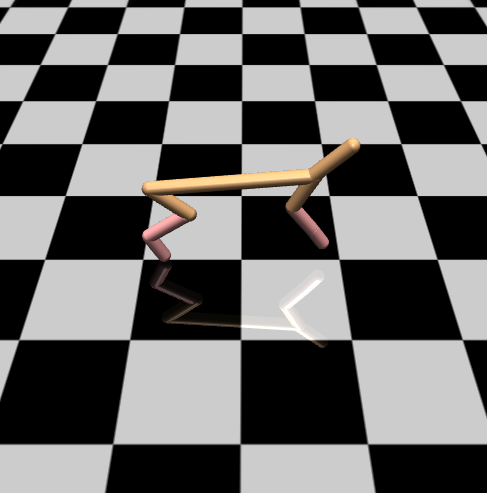
\includegraphics[width=\linewidth]{images/cheetah.png}
  \subcaption{HalfCheetah-v1}
\endminipage\hfill
\minipage{0.32\textwidth}
  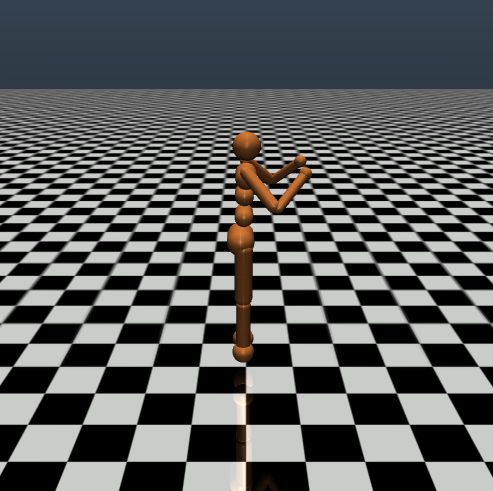
\includegraphics[width=\linewidth]{images/humanoid.png}
  \subcaption{Humanoid-v1}
\endminipage\hfill
\minipage{0.32\textwidth}%
  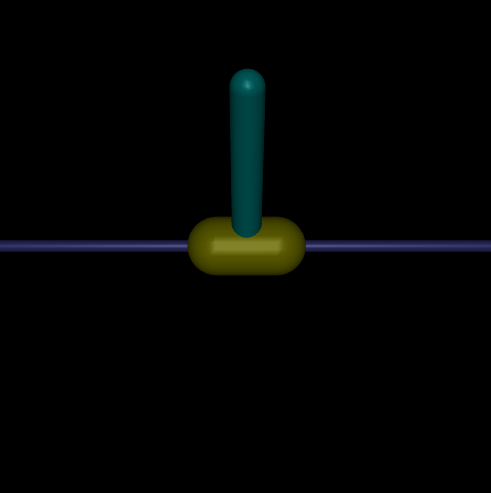
\includegraphics[width=\linewidth]{images/inv_pendulum.png}
  \subcaption{InvertedPendulum-v1}
\endminipage
\caption{Different MuJoCo environments}
\label{fig:mujoco_envs}
\end{figure}

\begin{figure}[!htb]
\centerline{

\includegraphics[width=0.5\textwidth]{images/snake.png}}
\caption{MuJoCo environment \emph{Swimmer-v1} we use in this thesis}
\label{fig:swimmer_env}
\end{figure}


In this chapter we introduced all required background knowledge and mathematical terms to understand the work of this thesis.
We started off by looking at the RL problem, defined its terms in mathematical language and then presented different approaches to solve it.
In the end the frameworks with the most impact on our work were also introduced.


The next chapter will present related work in this direction focusing on RL breakthroughs of the last few years and on how others approached the problem of \emph{Exploration vs Exploitation}.
